\chapter{Introduction and Search Strategy}

The Standard Model of particle physics (SM) is a well-established theory that describes the fundamental particles and how they interact. Despite its many successes, the SM has some important limitations. For example, it does not explain dark matter, does not include gravity, and has several free parameters such as why particles have the masses they do.
\\

The main goal of this experiment is to search for signs of  physics beyond the Standard Model (BSM). These BSM theories try to solve the SM’s problems by predicting new particles and forces. A popular example is a hypothetical heavy particle called the \( Z' \) boson. The $Z'$ theoretically decays into a top quark. The top quark is the heaviest elementary particle, with a mass of about \SI{173}{GeV} \cite{Workman2022}. It was discovered at the Tevatron collider in the United States. Since 2010, top quark studies have been carried out mainly at the Large Hadron Collider (LHC) by looking at proton-proton (\( pp \)) collisions that also produce \( t\bar{t} \) pairs and other particles.
\\

\begin{figure}[H]
    \centering
    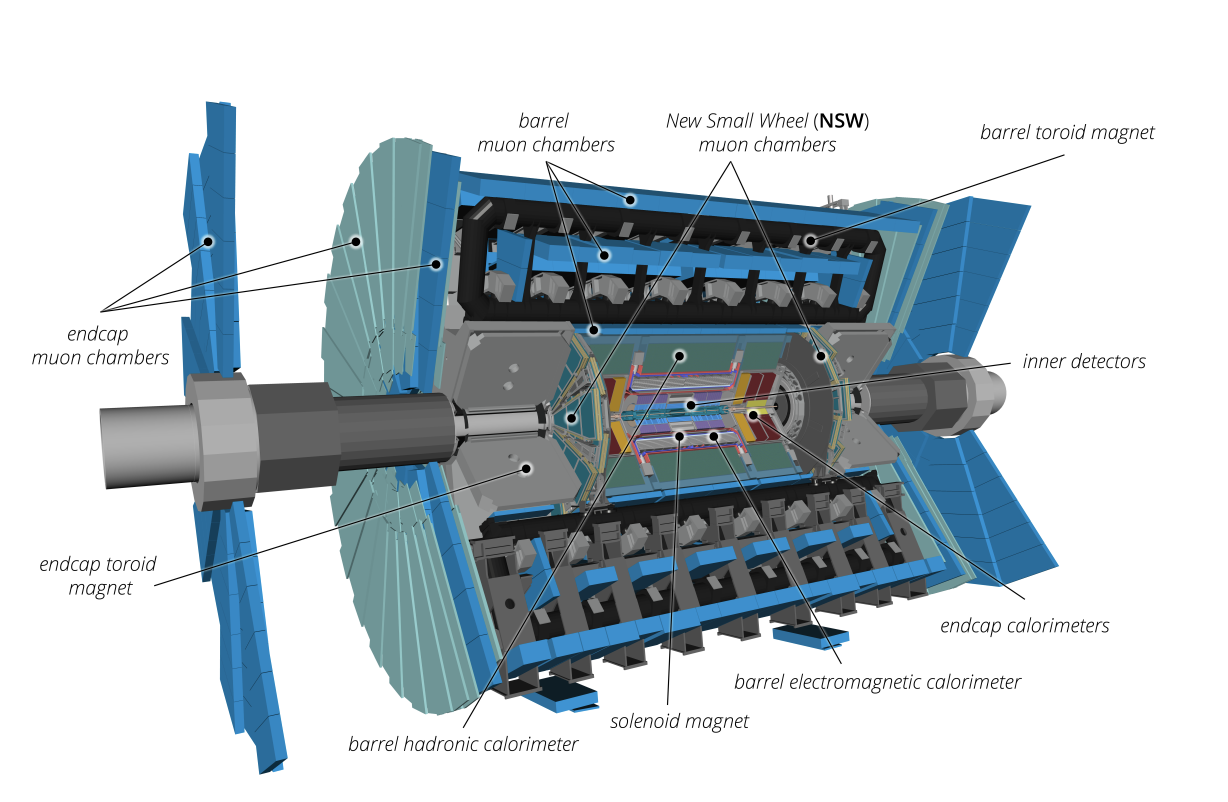
\includegraphics[width=0.6\linewidth]{Figure/atlas.png}
    \caption{The ATLAS detector showing the main sub-systems \cite{Aad2008}.}
    \label{atlas}
\end{figure}
\\

One of the main experiments studying \( t\bar{t} \) pairs events is the ATLAS detector at the LHC \ref{atlas}. ATLAS is a detector designed to detect almost any kind of new physics. It consists of several subsystems that work together to track particles and measure their energies and momenta. Although ATLAS does not detect top quarks directly, it observes the particles that result from top quark decays.
\\

The detector can be divided into four main parts: the inner detector, the calorimeters, the muon spectrometer, and the magnet system. The inner detector is the closest to the collision point and tracks charged particles. It includes a silicon pixel detector which has very high resolution useful for tagging \( b \)-jets, silicon strips, and a transition radiation tracker (TRT) that helps separate electrons and positrons by detecting transition radiation. Surrounding the inner detector are the calorimeters, which absorb particles and measure their energy.
\\

The muon spectrometer forms the outermost layer. Since muons can pass through the other layers without losing much energy. The inner detector is surrounded by a solenoid magnet that bends charged particle tracks allowing their momentum to be calculated. One limitation of detector including ATLAS is that it cannot directly detect neutrinos, as they interact only weakly and usually pass through undetected.
\\

In this experiment, \( t\bar{t} \) pairs are mainly produced through gluon-gluon fusion. We focus on the lepton+jets decay channel, where one top quark decays into a lepton (electron or muon) and a neutrino, and the other decays into jets, as illustrated in Figure \ref{tt-decay}.

\begin{figure}[H]
    \centering
    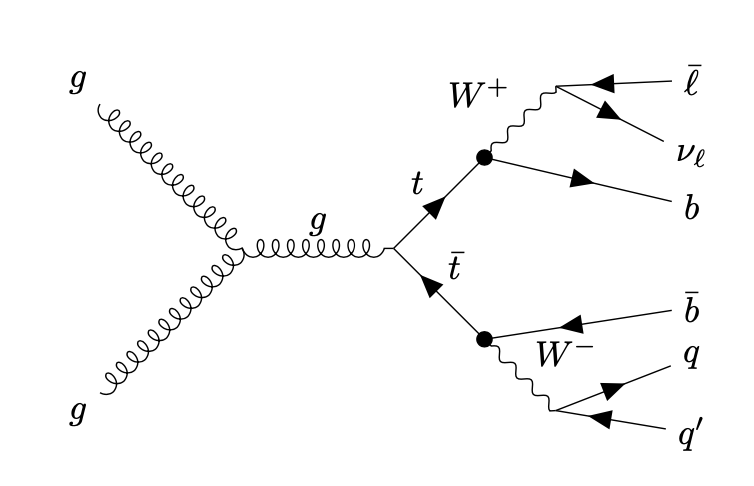
\includegraphics[width=0.5\linewidth]{Figure/tt-decay.png}
    \caption{Feynman diagram showing \( t\bar{t} \) production through gluon-gluon fusion and decay in the lepton+jets channel.}
    \label{tt-decay}
\end{figure}

This channel is chosen because it provides a good balance between background and signal visibility. To account for the presence of neutrinos, missing transverse momentum (\( E_T^{\text{miss}} \)) is used as a key observable. To identify jets originating from \( b \)-quarks, \( b \)-tagging algorithms are applied. To perform the analysis, events are selected using criteria that enhance the signal over the background. These include requirements on the number of jets, a high-\( p_T \) lepton, and missing transverse energy (\( E_T^{\text{miss}} \)) to account for neutrinos. Backgrounds are estimated using Monte Carlo (MC) simulations and validated with real data. A final discriminant is used in a statistical test to search for deviations from the Standard Model prediction. A signal in this channel would suggest new physics.



